\documentclass{article}

\usepackage{tabularx}

% NOTE: To put equations in their environment we need either `float` or
% `caption`.  We use float to put equations and other environments exactly
% where they appear in the code with the `H` placeholder, and for that we
% redefine the `equ` environment sort of twice, so this is a bit flaky but
% it works.
\usepackage{caption}
\DeclareCaptionType{equ}[][]
\captionsetup[equ]{name=נוסחא}
\usepackage{float}
\floatstyle{plain}
% https://www.overleaf.com/learn/latex/Positioning_of_Figures
\newfloat{equ}{H}{eq}[section]
\floatname{equ}{נוסחא}

\DeclareCaptionType{graph}[][]
\captionsetup[graph]{name=גרף }

% to includegraphics
\usepackage{graphicx}

% to fix itemize lists:
% https://tex.stackexchange.com/a/53453/125609
\usepackage{enumitem}
\setlist[itemize,1]{label={\fontfamily{cmr}\fontencoding{T1}\selectfont\textbullet}}

% Links
\usepackage{hyperref}
\hypersetup{colorlinks = true,
	citecolor = gray,
	linkcolor = red,
	citecolor = green,
	filecolor = magenta,
	urlcolor = cyan
}

% To include plots by matplotlib
\usepackage{pgfplots}
\pgfplotsset{compat=newest}
% Note we use resizebox as explained here through out the document https://tex.stackexchange.com/a/582956/125609

% Language
\usepackage{polyglossia}
\setdefaultlanguage{hebrew}
\setotherlanguage{english}
\usepackage{hebrewcal}

\usepackage[
backend=biber,
isbn=false,
style=numeric,
doi = false,
sorting=ynt
]{biblatex}
% Seems to be a recommended package but it makes quotes in bibliography at the
% end appear with a question mark instead of `"`.
%\usepackage{csquotes}
\addbibresource{references.bib} % Imports bibliography file

% Fonts
\setmainfont{David CLM}
\setsansfont{Liberation Sans}
\setmonofont{Liberation Mono}
\newfontfamily\hebrewfont{David CLM}[Script=Hebrew]
\newfontfamily\hebrewfontsf{Liberation Serif}[Script=Hebrew]
\newfontfamily\hebrewfonttt{Liberation Mono}[Script=Hebrew]

\title{
	מדידת רמות אנרגיה של מתכות באמצעות ספקטרוסקופית
	\textenglish{X-ray}
}
\author{
שרה לחצר ודורון בכר \\
הפקולטה לפיזיקה, הטכניון - מכון טכנולוגי לישראל.
}
\date{\today}

\begin{document}
\maketitle

\begin{abstract}
% TODO
\end{abstract}
\section{מבוא}

אלקטרונים באטומי מתכות נמצאים במצבים קוונטיים הנקראים אורביטלים. לכל אלקטרון בכל אורביטל יש אנרגיה מסוימת ואוסף האנרגיות הזה אופייני ושונה בין מתכות שונות. באופן דומה למודל אטום המימן אותו ניתן לחשב באופן אנליטי, גם במתכות לאורביטלים העליונים יש אנרגיה גבוהה יותר מלאורביטלים התחתונים
($\frac{1}{n^2}\sim$).

אלקטרונים באורביטלים החיצוניים ניתנים ליינון באמצעות
"התנגשות"
אלקטרונים אחרים עם אנרגיה קינטית מתאימה. כאשר האטום מיונן, קיים סיכוי שאלקטרון מאורביטל אחר יתפוס את מקומו של האלקטרון שברח. המעבר של האלקטרון בין האורביטל התחתון לעליון כרוך בירידה באנרגיה, ועל כן בפליטה של פוטון לפי הקשר
$\Delta E = h \nu_{\gamma}$
כאשר
$h$
קבוע פלנק
ו-
$\nu_{\gamma} = \frac{c}{\lambda}$
הינו תדר הפוטון, עם
$c$
מהירות האור ו-
$\lambda$
אורך הגל של הפוטון. אנרגיות מעבר אלו במתכות הינן בתחום ה-
\textenglish{X-ray}
כלומר בין
$145 eV$
ל-
$124 keV$.

מודל זה מניח כי יינון של אטום לא גורר שינויים משמעותיים באורביטלים והאלקטרון שתופס את מקומו של האלקטרון שברח מקבל בקירוב את האנרגיה שהייתה לאלקטרון שברח באורביטל הגבוהה יותר. אנרגיות אורביטלים אלו יכולות להיות שונות בגלל אנרגיה אינטראקציה בין אלקטרונים שונים, והעובדה כי המיסוך על המטען החשמלי של הגרעין שונה בין האטום המיונן ובין האטום הניטרלי.

\subsection{מערכת הניסוי}

השתמשנו בערכת ניסוי של חברת
\textenglish{PHYWE}\begin{english}\footnote{\url{https://www.phywe.com/physics/modern-physics/x-ray-physics/}}\end{english}
ובחרנו בשפורפרת היורה אלקטרונים העשויה מ-
\textenglish{molybdenum}. שימוש באלקטרונים ליינון מתכות יכול לגרום למצב בו אטומי המתכת מיוננים (ולכן עם מטען חיובי), והאלקטרונים הנוספים המגיעים מהמקור משנים את כיוון המהירות שלהם ומאבדים אנרגיה קינטית. איבוד אנרגיה זה מתבטא גם כן בפוטונים הנפלטים ונקלטים בגלאי. קרינה זו נקראת
\textenglish{bremsstrahlung},
היא בתחום ה-
\textenglish{X-ray}
גם כן,
והיא אופיינית לשפורפרת בה בחרנו
(\textenglish{molybdenum}).
הטווח של קרינה זו רציף בניגוד לספקטרום הפליטה של המתכות אותו מדדנו. על כן היא איננה חלק מתוצאות הניסוי המוצגות בתוצאות.

באיור
\ref{fig:experiment_scheme}
הלקוח מתוך אתר היצרן, ניתן לראות צילום של המערכת. 
הגלאי המופיע בתמונה התחבר לרכיב הנקרא
\textenglish{MCA - Multi-Channel-Analyzer},
גם כן מוצר של
\textenglish{PHYWE}
שבנה היסטוגרמה של כמות הקרינה כתלות במספר הערוץ של הגלאי, לכל אורך הזמן בו פעלה שפורפרת. כל ערוץ בו מקבל פוטונים באנרגיה מסוימת ולכן הציר המייצג את מספר הערוץ לינארי לציר האנרגיה.

\begin{figure}
    \centering
    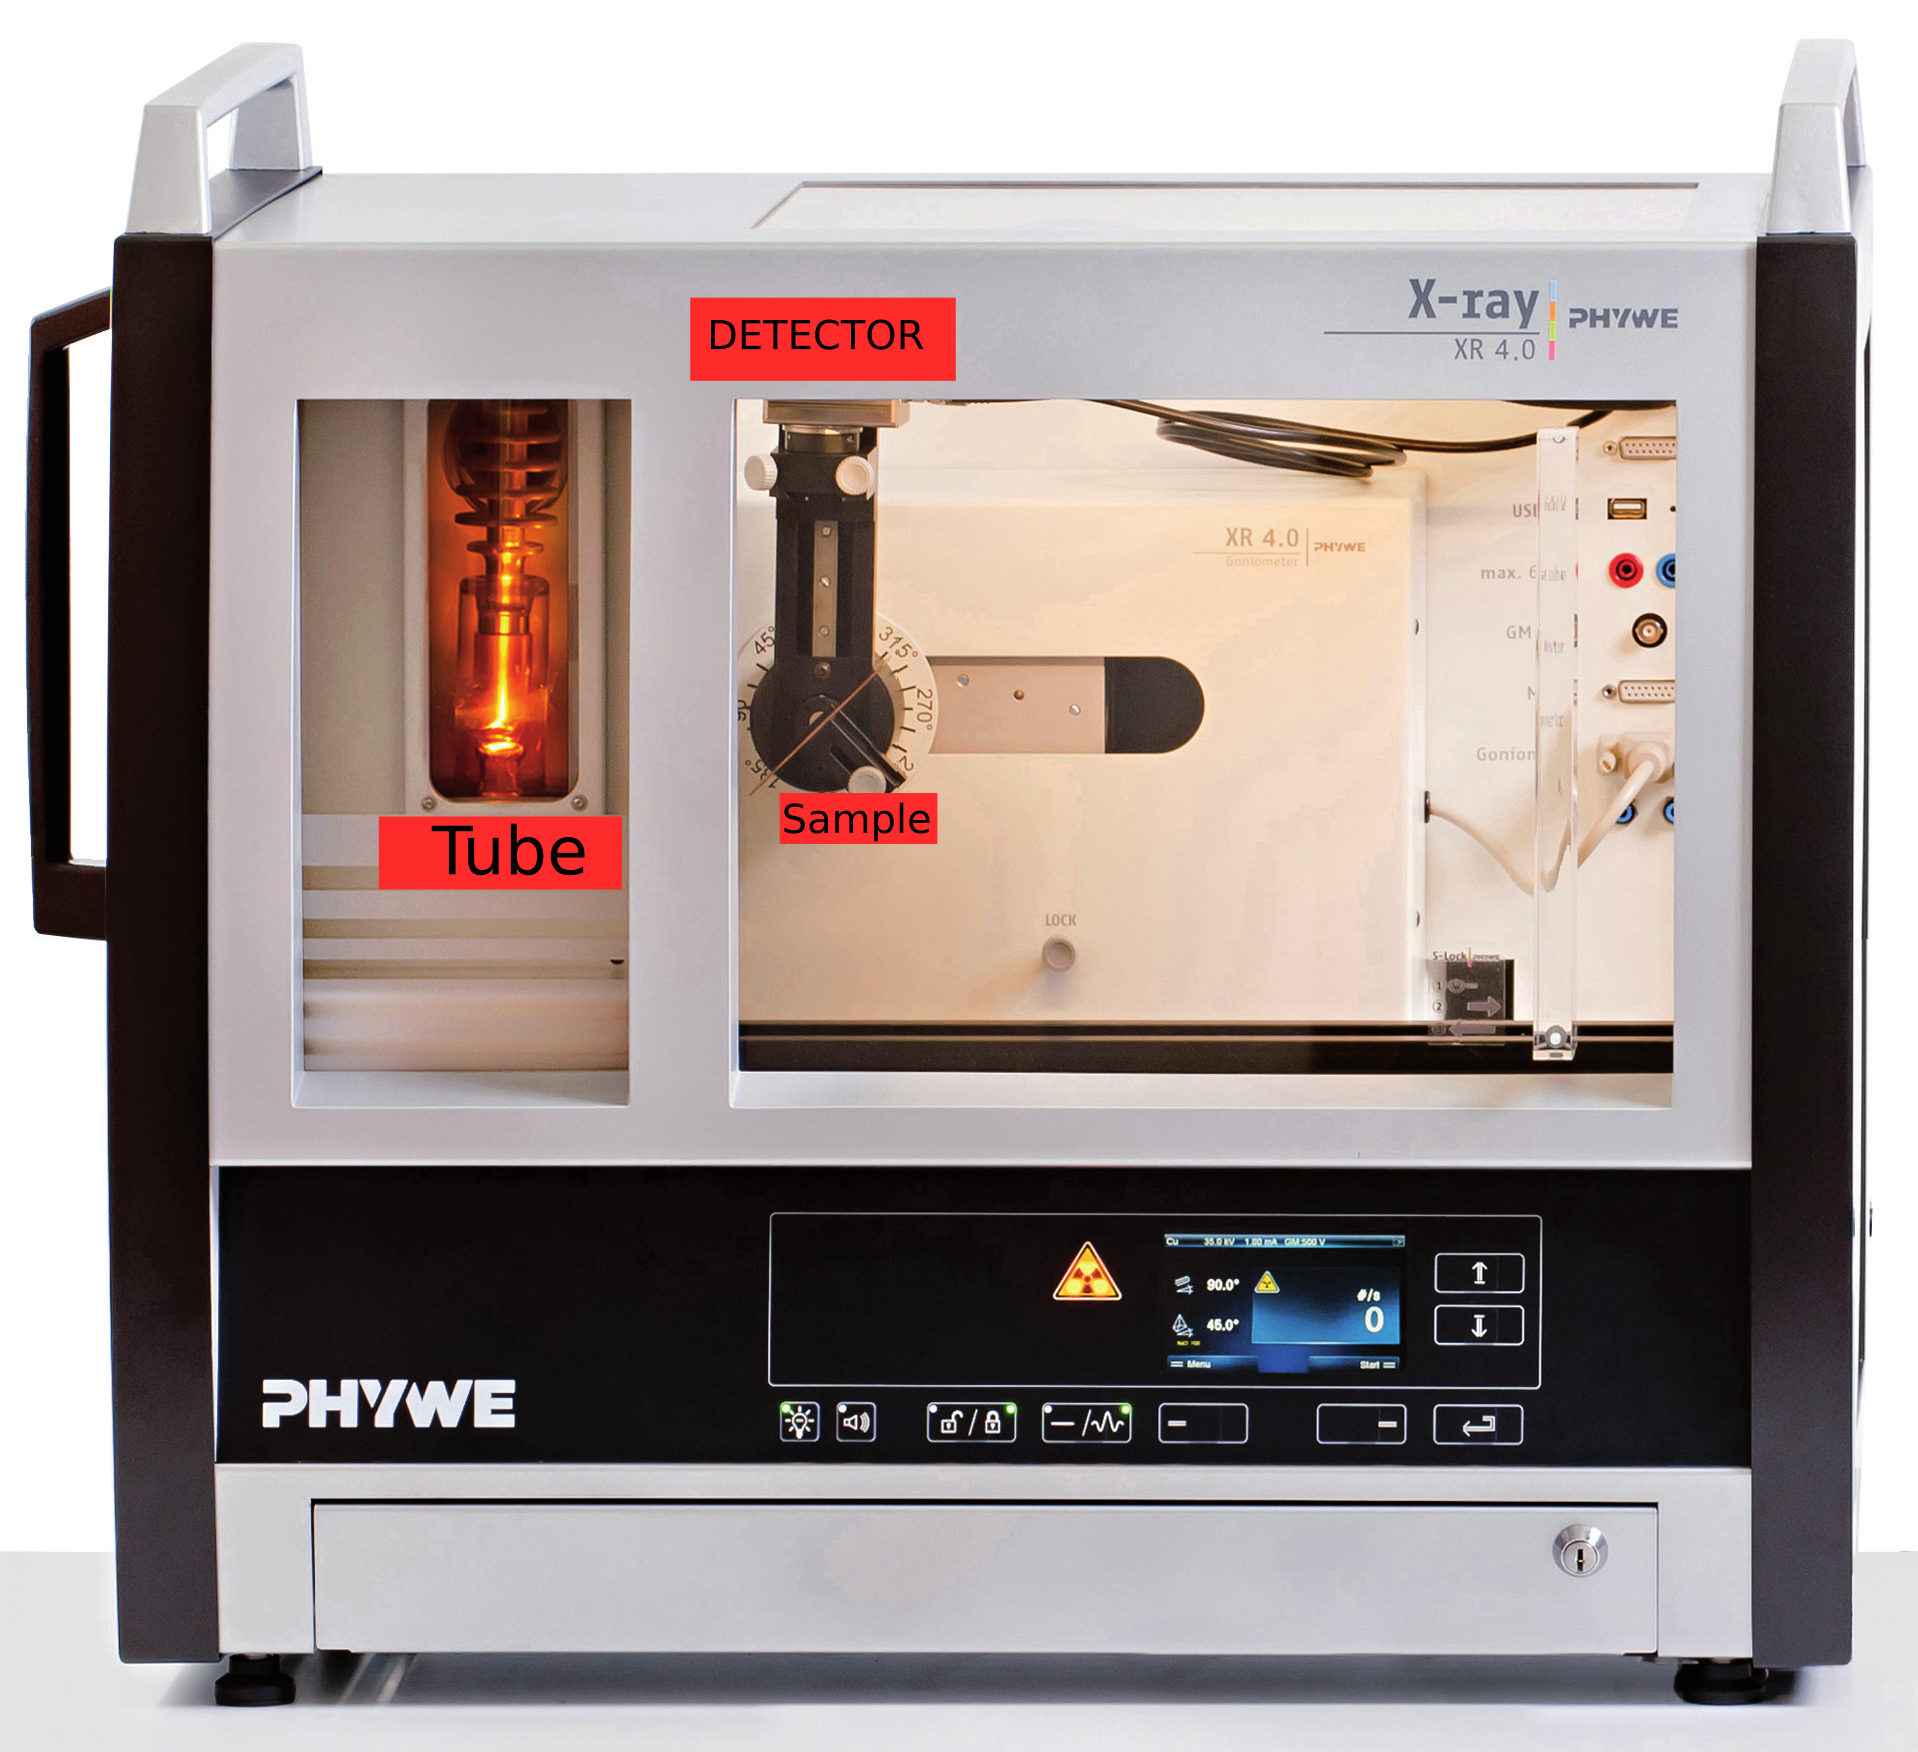
\includegraphics[width=\textwidth]{./system.png}
    \caption{
    איור של מערכת הניסוי, בטקסט על רקע אדום - גלאי הקרינה, הדגימה והשפורפרת.
    }
    \label{fig:experiment_scheme}
\end{figure}

השתמשנו במדידות של המופיעות ב-
\cite{xrayBooklet}
כדי לכייל את מספרי הערוצים לציר האנרגיה. הסתכלנו על הערוצים בהם מתקבלים נקודות מקסימום בהיסטוגרמה והתאמנו אותן לאנרגיות בהן המתכות שבדקנו פולטות/בולעות, בהתחשב בעוצמות היחסיות המופיעות בטבלאות גם כן. המתכות בהן השתמשנו וההיסטוגרמות מופיעות בגרף
% TODO: Add ref to graph

בנוסף זיהינו שמטבע של חצי ש"ח ישראלי עשוי מנחושת באמצעות השוואה של ההיסטוגרמה של הנחושת שמצאנו והשוואתה להיסטוגרמה של המטבע.

השתמשנו בכיול לעיל כדי לזהות את ההרכב הכימי של כמה מוצקים ובדקנו האם ישנה התאמה בין המרכיבים הכימיים של הגבישים לעיל לחומרים שההיסטוגרמה שלהם מתאימה לאנרגיות המופיעות ב-
\cite{xrayBooklet}.

\section{תוצאות}

\begin{graph}[H]
    \centering
    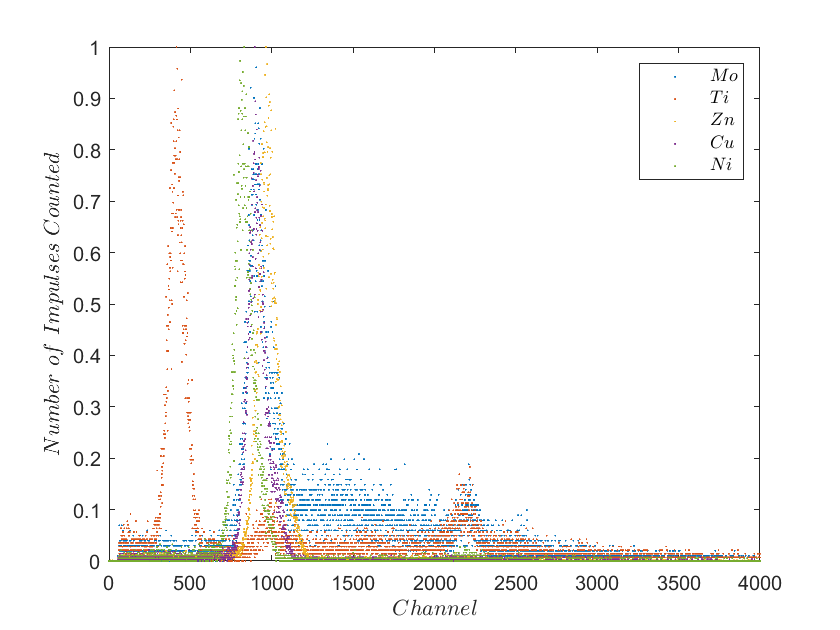
\includegraphics[width=\textwidth]{specNormlized.png}
    \caption{
    היסטוגרמות של בליעת קרינת
    \textenglish{X-ray}
    בגלאי למתכות שונות.
    }
    \label{graph:histograms}
\end{graph}

בגרף
\ref{graph:histograms}
ניתן לראות את ההיסטוגרמות של המתכות השונות שדגמנו, כאשר הציר האופקי אינו מכוייל לציר אנרגיה. זיהינו את המקומות בהם הופיעו המקסימות בכל מתכת ויצרנו את גרף הכיול שלהלן:

\begin{graph}[H]
    \centering
    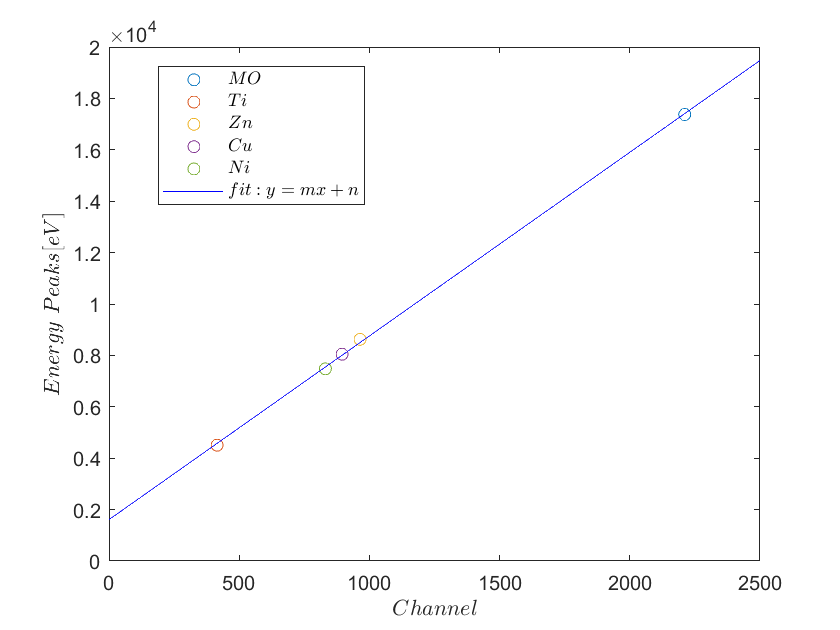
\includegraphics[width=\textwidth]{calibration.png}
    \caption{
    הקשר הלינארי בין האנרגיות למספר הערוץ ב-
    \textenglish{MCA}.
    }
    \label{graph:MCA-energies}
\end{graph}

ביצענו התאמה לינארית וקיבלנו ששיפוע הגרף הינו 
$m = 7.1 \pm 0.2 [\frac{eV}{channel}]$
והאיבר החופשי 
$n = 1608 \pm 279 [eV]$,
טיב ההתאמה היה 
$R^2 = 0.9997$.

השתמשנו בקשר הלינארי המופיע ב-
\ref{graph:MCA-energies}
כדי לזהות את ההרכבים של הגבישים שלהלן:
% TODO: Make the list here more accurate, add the chemical elements composing them.
\begin{enumerate}
    \item Hamatit
    \begin{graph}[H]
    \centering
    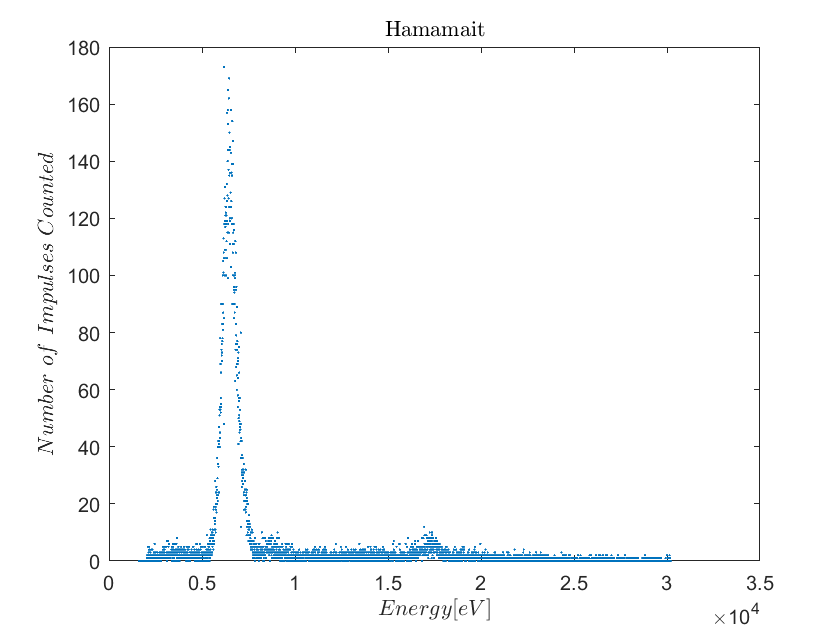
\includegraphics[width=\textwidth]{Hamamit.png}
    \caption{מדידת ספקטרום האנרגיה עבור 
    \textenglish{Hamatit}.
    }
    \label{graph:Hamatit-spec}
    \end{graph}
    התקבל פיק יחיד בערך
    $E_{Hamatit} = 6453 \pm 50 [eV]$
    \item Descloizit
    \begin{graph}[H]
    \centering
    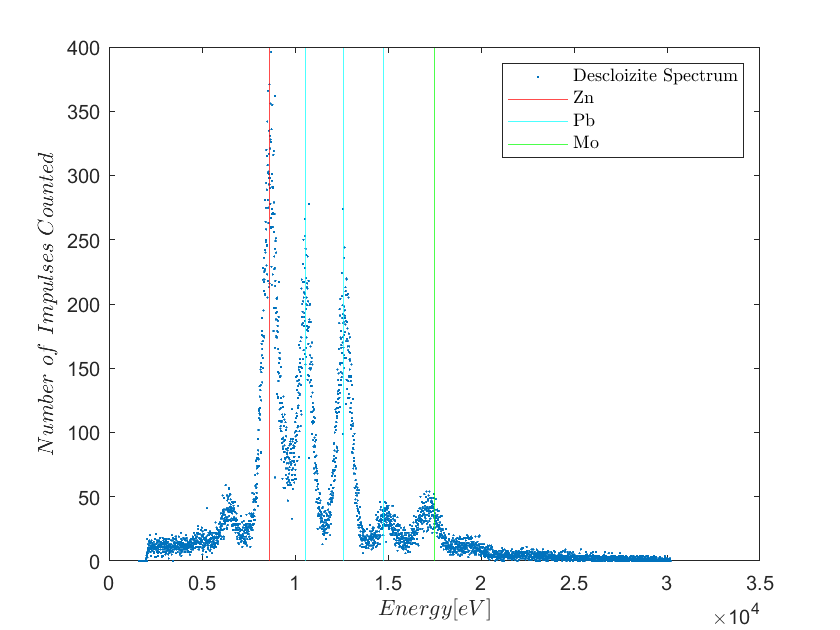
\includegraphics[width=\textwidth]{Descloizit.png}
    \caption{מדידת ספקטרום האנרגיה עבור 
    \textenglish{Descloizit}
    }
    \label{graph:Descloizit-spec}
    \end{graph}
    התקבלו שלושה פיקים באנרגיות הבאות:
    \begin{enumerate}
    \item $E_{Descloizit}^1 = 8625 \pm 110 [eV]$
    \item $E_{Descloizit}^2 = 10748 \pm 231 [eV]$
    \item $E_{Descloizit}^3 = 12556 \pm 158 [eV]$
    \end{enumerate}
\end{enumerate}
%השגיאות הוערכו ידנית לפי טווח הפיק.
% TODO: Write another paragraph about the fitting done for the materials above

\section{דיון בתוצאות}

\section{מסקנות}

\section*{סימוכין}
\begin{english}
\printbibliography[heading=none]{}
\end{english}

\end{document}
